%% You can use this file to create your answer for Exercise 1.  
%% Fill in the places labeled by comments.
%% Generate a PDF document by with the command `pdflatex ex1'.

\documentclass[11pt]{article}

\usepackage{fullpage}
\usepackage{amsmath,amsopn}
\usepackage{graphicx}
\usepackage{color}
\usepackage{verbatim}
\usepackage{setspace}
\usepackage{gensymb}
\usepackage{float}
\usepackage{pgfplots}
\usepackage{pgfplotstable}
\pgfplotsset{compat=1.16}
\usepackage[normalem]{ulem}
%\usepackage[dvips,bookmarks=false,colorlinks,urlcolor=blue,pdftitle={
\usepackage{caption}
\usepackage{subcaption}
\usepackage{amssymb}
\usepackage{amsfonts}
\usepackage{amsthm}
\usepackage{comment}
\usepackage{times}
\usepackage{listings}
\usepackage{enumerate}
\usepackage{courier}
\usepackage{hyperref}
\usepackage{xcolor}
\usepackage{verbatimbox}
\usepackage{tikz}
\usepackage{tikzscale}
\usepgfplotslibrary{groupplots}
\usepackage{float}
\usepackage{natbib}

\def\vO{{\bf O}}
\def\vP{{\bf P}}
\def\vp{{\bf p}}
\def\vx{{\bf x}}
\def\vl{{\bf l}}
\def\mS{{\bf S}}
\def\mT{{\bf T}}
\def\mH{{\bf H}}
\def\mA{{\bf A}}
\def\tx{{\tilde{\bf x}}}
\def\ta{{\tilde{\bf a}}}
\def\tb{{\tilde{\bf b}}}
\def\tc{{\tilde{\bf c}}}
\def\hn{{\bf \hat{n}}}
\def\hv{{\bf \hat{v}}}
\def\hh{{\bf \hat{h}}}
\def\vh{{\bf h}}
\def\vs{{\bf s}}
\def\hs{{\bf \hat{s}}}
\newcommand{\R}{\mathbb{R}}
\newcommand{\ud}{\,\mathrm{d}}

%% Values that are specific to a particular term
\newcommand{\thisterm}{Fall 2023}

\newcommand{\dateassigned}{Wed., Sep. 13}

%% Printed form of home page that students should use
\newcommand{\visiblecoursehome}{http://www.cs.cmu.edu/\textasciitilde{}418}

%% Link to home page that will stay valid
\newcommand{\actualcoursehome}{http://www.cs.cmu.edu/afs/cs.cmu.edu/academic/class/15418-s23/www}

\newcommand{\datedueregistered}{Wed.,~Sep.~27}

%% Page layout
\oddsidemargin 0pt
\evensidemargin 0pt
\textheight 600pt
\textwidth 469pt
\setlength{\parindent}{0em}
\setlength{\parskip}{1ex}

%% Colored hyperlink 
\newcommand{\cref}[2]{\href{#1}{\color{blue}#2}}
\newcommand{\todo}[1]{[\textcolor{red}{\textit{TODO: }{#1}}]}

%% Customization to listing
\lstset{basicstyle=\ttfamily,language=C++,morekeywords={uniform,foreach}}

%% Enumerate environment with alphabetic labels
\newenvironment{choice}{\begin{enumerate}[A.]}{\end{enumerate}}
%% Environment for supplying answers to problem
\newenvironment{answer}{\begin{minipage}[c][1.0in]{\textwidth}}{\end{minipage}}
\newenvironment{answer2}{\begin{minipage}[c][1.0in]{\textwidth}}{\end{minipage}}

\begin{document}
\begin{center}
\LARGE
15-418/618 \thisterm{} Project Milestone Report
\\ 
Sparse Attention in CUDA
\end{center}
\begin{flushright}
{\large\bf Full Names: Sarah Di, Jinsol Park\makebox[2in][l]{
%% Put your name on the next line

}}

{\large\bf Andrew IDs: sarahdi, jinsolp\makebox[2in][l]{\tt
%% Put your Andrew ID on the next line

}}
\end{flushright}

{\large\bf Project Page URL: \url{https://github.com/disarah/15618\_Project}\makebox[2in][l]{
%% Put your name on the next line

}}


\section{Work Completed so far}
% (1-2 paragraphs)
% • Summarize the work that you have completed so far. : Sarah: breakdown / Jinsol write in bulletpoints
\subsection{Summary of work}

Following the work of \citet{child2019generating} with Sparse Attention Transformers, we first validate the motivation for sparse attention with empirical data. The graphs which confirm that attention is a performance bottleneck can be seen in the Preliminary Results section.

\begin{figure}[h]
  \centering
  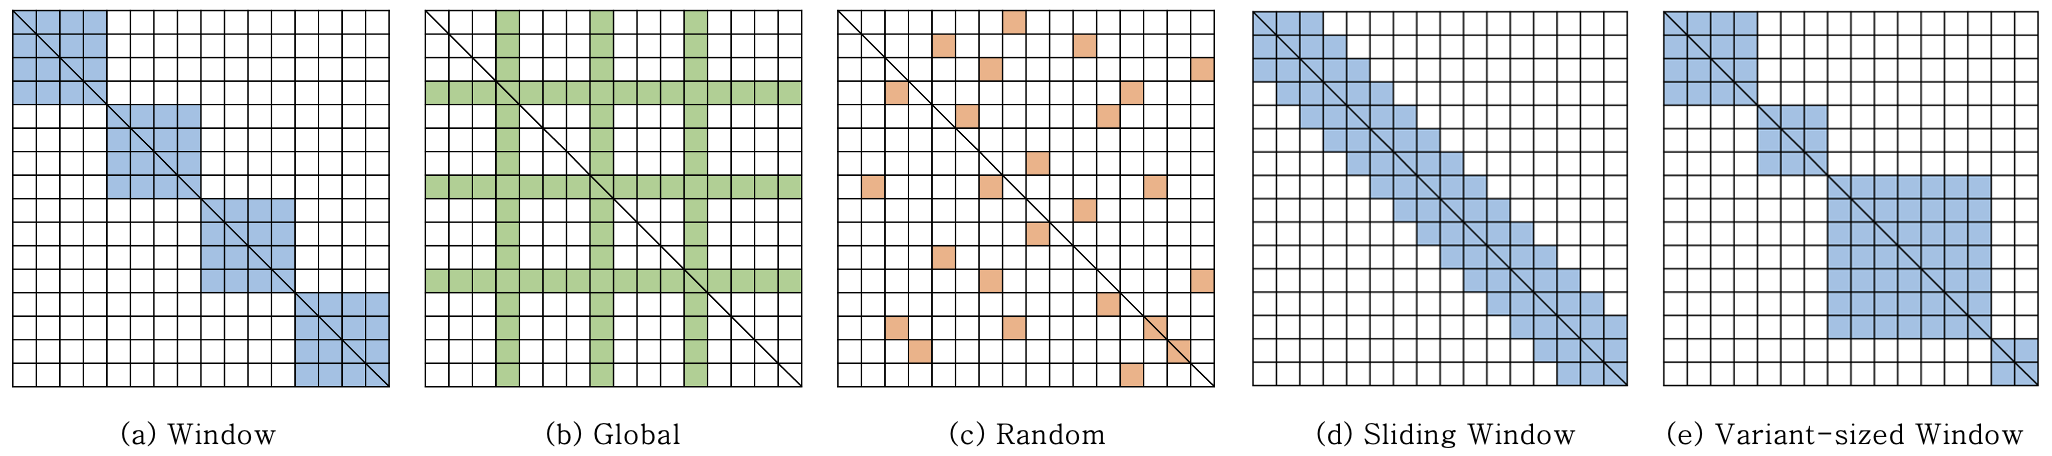
\includegraphics[width=170mm]{figures/building_block.png}
  \caption{Different factorization methods of sparse attention.  Each connectivity matrix shows whether an $i^{th}$ token (row) of a sequence refers to a $j^{th}$ token (column) to compute an attention score. These can be combined to be a single sparse attention method.}
 \label{fig:bulding_block}
\end{figure}

We implemented the naive attention and the sparse attention on CPU and CUDA. For the naive attention, we implemented general matrix multiplication and the softmax using a tiling scheme to exploit shared memory efficiently.\\
For this milestone, we focused on the window attention method as seen in (a) of \autoref{fig:bulding_block} for sparse attention. Since query and key matrices are dense but the resulting attention scores matrix is sparse, we cannot use general matrix multiplication. Instead, we implemented a \texttt{MultiHeadDDS} kernel, which performs dense $\times$ dense = sparse matrix multiplication based on the given window size. We also implemented a \texttt{MultiHeadSoftMaxSparse} kernel, which performs sparse softmax on the sparse attention scores matrix. Finally, we also have a \texttt{MultiHeadSDD} kernel to perform matrix multiplication between the sparse attention scores matrix and the dense value matrix, returning a dense matrix as the final output. All matrix multiplication kernels use tiling optimizations, and uses the window size configuration to efficiently exploit shared memory.

\subsection{Being on Schedule}
% • Describe how you are doing with respect to the goals and deliverables stated in your proposal. Do you still believe you will be able to produce all your deliverables? If not, why? What about the ”nice to haves”? In your milestone writeup we want a new list of goals that you plan to hit for the poster session. - be general...  

We believe we will be able to finish all ``plan to achieve" goals. We also plan to work on the ``hope to achieve" goals for the remaining time. A specified schedule for the rest of the semester is in \autoref{sec:revised-schedule}

\subsection{Plans for the Poster Session}
At the poster session, we are planning on showing multiple graphs showing the speedup of our implementations with respect to sequence length. Additionally we will include visualizations of the final tiling methods used and visualizations of how shared memory is exploited in our CUDA implementations.

\subsection{Preliminary Results}
\begin{figure} [H]
\pgfplotstableread{
    Label SelfAttention SelfOutput Intermediate Output topper
    128 0.079665  0.019992 0.084192 0.073205 0.001
    256 0.300243  0.040303 0.153612 0.147656 0.001
    512 0.545014 0.078534 0.322093 0.282523 0.001
    1024 3.854414 0.193473 0.686376 0.707752 0.001
        }\testdata
    \centering
    \includegraphics[width=9cm]{layersPlot.tikz}
    \caption{Computational Times for layers in a transformer vs Sequence Length}
    \label{fig:timing}
\end{figure}
In \autoref{fig:timing}, we show the computational time of the layers present within a BERT encoder scaled by the sequence length of the inputs (ranging from 128 to 1024). Our visualization confirms that the computation time of the encoder's attention layer, as shown in green, scales quadratically with respect to sequence length, and also that is takes up a large proportion of the computation time. 
We also include the computational times of other layers of the encoder, such as the Intermediate and Output (Add \& Norm) layers, as shown in red and orange respectively, which combined comprise the Feed Forward part of an encoder. The SelfOutput layer, shown in blue, represents the Add \& Norm Layer of Self Attention.

\begin{figure} [H]
\centering
\begin{subfigure}{.5\textwidth}
  \centering
  \includegraphics[height=8cm, width=\linewidth]{attentionPlotCPU.tikz}
  \label{fig:attnCPU}
\end{subfigure}%
\begin{subfigure}{.5\textwidth}
  \centering
  \includegraphics[height=8cm, width=\linewidth]{attentionPlotGPU.tikz}
  \label{fig:attnGPU}
\end{subfigure}
\caption{Execution Time vs Sequence Length for CPU and GPU implementations}
\label{fig:attnPlots}
\end{figure}

\autoref{fig:attnPlots} shows the execution time of attention on GPU for different attention methods. We measured the execution time for sequence lengths 128, 256, 512, and 1024. It can be observed that the GPU Naive Attention scales quadratically with sequence length, while the GPU Sparse Attention implementation (with window size 16) scales linearly with sequence length. Also, it takes much less time compared to the full naive attention.

\begin{table}[h!]
\centering
 \begin{tabular}{|c || c c c c|} 
 \hline
  SeqLen & GPU Sparse & GPU Naive & CPU Sparse & CPU Naive \\
 \hline 
    128 & $\times$1 & $\times$5.15 & $\times$51.02 & $\times$476.46 \\
    256 & $\times$1 & $\times$10.63 & $\times$87.01 & $\times$1238.01 \\
    512 & $\times$1 & $\times$27.88 & $\times$181.65 & $\times$3706.75 \\
    1024 & $\times$1 & $\times$143.32 & $\times$332.90 & $\times$8652.24 \\
    % 2048 & 13.631169 & 0.332429 & 1.277496 & 1.172507 \\
 \hline
 \end{tabular}
 \caption{Speedup of GPU window sparse implementation compared to other implementations}
 \label{table:speedup}
\end{table}

\autoref{table:speedup} provides further information about the execution time on CPU Sparse and Naive Attentions. We provide a speedup brought by GPU Sparse Attention compared to each implementation for different sequence lengths.


\subsection{Remaining Challenges}
% • List the issues that concern you the most. Are there any remaining unknowns (things you simply don’t know how to solve, or resource you don’t know how to get) or is it just a matter of coding and doing the work? If you do not wish to put this information on a public web site you are welcome to email the staff directly. : Jinsol - apart from window upcoming sparse attention diffcicult to optimize (think of other ways to use shared mem) + NSight

We plan to implement additional sparse attention mechanisms from \autoref{fig:bulding_block}. Unlike the window attention which intuitively aligns well with our tiling optimization, other versions are more difficult to optimize by exploiting shared memory. \\
Also, one of our ``hope to achieve" plans is to use CUDA profiling tools (such as NSight Compute or Systems). Since neither of us are familiar with these tools, we will be treating this as an opportunity to learn, even if our kernel profiling results are unsuccessful.

\section{Revised Schedule}
\label{sec:revised-schedule}
% \section{Schedule}
Our finalized schedule for the remainder of the semester is as follows:
\begin{center}
\begin{tabular}{ |c|c|c| } 
 \hline
 Time & Plan & Person\\ 
 \hline
 12/03 & Milestone Report Due  & Jinsol \& Sarah\\ 
 - & Have 1 CUDA implementation \& benchmark & - \\
 12/06 & Read literature about different sparse attention mechanisms & Jinsol \& Sarah\\ 
 12/10 & Additional CUDA implementations \& optimizations & Jinsol \& Sarah\\
 - & Complete Background on Final Report  & - \\
 12/13 & Finish Experiments/Discussion on Final Report & Jinsol \& Sarah\\
 12/14 & Final Report Due & Jinsol \& Sarah\\ 
 - & Finish Poster  & - \\
 12/15 & Poster Session  & - \\
 \hline
\end{tabular}
\end{center}

\bibliographystyle{unsrtnat}
\bibliography{MilestoneReport/milestone}
\end{document}